\documentclass{article}
% ICLR 2027 double-blind SUBMISSION build. The arXiv build lives in main.tex.
% NOTE: iclr2027_conference.{sty,bst} here are the 2026 files with the year
% updated; replace them with the official ICLR 2027 template before submitting.
\usepackage{iclr2027_conference,times}
\usepackage{natbib}
\usepackage{amsmath,amssymb}
\usepackage{booktabs}
\usepackage{graphicx}
\usepackage{hyperref}
\usepackage{url}
\usepackage{algorithm}
\usepackage{algorithmic}
\usepackage{wrapfig}

\newif\ificlrcompact\iclrcompacttrue   % ICLR: defer big floats to the appendix
% Floats inline in the arXiv build, deferred to the appendix in the page-limited
% ICLR build. Defined once; placed by the \ificlrcompact flag.
\newcommand{\AlgCompSel}{%
\begin{algorithm}[!htb]
\footnotesize
\caption{Compensated Selection (\textsc{hybrid\_rs})}
\label{alg:compsel}
\begin{algorithmic}[1]
\REQUIRE donor weights $W_L$; frozen-corpus activation variances and second
moments $\Sigma$; target shape (residual $d'$, head dim, MLP width, block map)
\ENSURE installable small-model weights (no target-model access)
\STATE $\mathcal{R} \gets$ top-$d'$ residual features by mean-over-layer activation variance \COMMENT{one global basis}
\FOR{each kept block $b$}
  \STATE $\mathcal{K}_{qk} \gets$ frequency-matched rotary pairs (stride $2$) $\cup$ top non-rotary dims by $\lVert q\rVert{+}\lVert k\rVert$
  \STATE $\mathcal{K}_{vo} \gets$ top head dims by $\lVert V_{\text{row}}\rVert\cdot\lVert O_{\text{col}}\rVert$ \COMMENT{whole heads if head count shrinks}
  \STATE $\mathcal{K}_{mlp} \gets$ top units by $\lVert\text{up}_{\text{row}}\rVert\cdot\lVert\text{down}_{\text{col}}\rVert$
  \STATE slice $W_L$ block $b$ to $(\mathcal{R},\mathcal{K}_{qk},\mathcal{K}_{vo},\mathcal{K}_{mlp})$; LayerNorms and biases ride along
  \STATE $O' \gets \text{LScomp}(O,\,\Sigma_{\text{attn-in}},\,\mathcal{K}_{vo})$;\; $\text{MLP\_down}' \gets \text{LScomp}(\text{MLP\_down},\,\Sigma_{\text{mlp-in}},\,\mathcal{K}_{mlp})$ \COMMENT{Eq.~\ref{eq:lscomp}, function lever}
  \IF{rescale}
    \STATE multiply LN-fronted read-in paths $Q,K,V,\text{MLP\_up}$ (and output embedding) by $\sqrt{d_{\text{in}}/d_{\text{in}}'}$ \COMMENT{dynamics lever}
  \ENDIF
\ENDFOR
\RETURN assembled small model
\end{algorithmic}
\end{algorithm}
}
\newcommand{\TabPredictor}{%
\begin{table}[!htb]
\centering
\footnotesize
\caption{Tests 3--4 (learnability and transfer). Patch-predictor error reduction
over predicting zero vs.\ a label-shuffled control; 1000-sample bootstrap CI on
the real$-$control gap. No predictor beats zero or separates from its control.}
\label{tab:predictor}
\begin{tabular}{llcccc}
\toprule
Setting & Predictor & Reduction & Shuffle & Gap CI$_{95}$ & $p$ \\
\midrule
Held-out layers (1.4B$\to$410M) & linear  & $-0.0004$ & $-0.0004$ & $[-0.0000,-0.0000]$ & 0.99 \\
                                & MLP-512 & $-0.0003$ & $-0.0003$ & $[-0.0000,-0.0000]$ & 1.00 \\
\midrule
Transfer (410M$\to$160M)        & linear  & $-0.0004$ & $-0.0004$ & --- & 1.00 \\
                                & MLP-512 & $-0.0003$ & $-0.0002$ & --- & 1.00 \\
\bottomrule
\end{tabular}
\\[3pt]
{\footnotesize CIs are reported for the in-pair held-out test only; the transfer
test reports $p$ (M4). Reductions are negative because no predictor improves on
predicting zero.}
\end{table}
}


% \iclrfinalcopy is intentionally OFF: anonymous authors + line numbers.

\title{Wiring Beats Blending: What Transfers Between\\Transformer Sizes --- and What Doesn't}

\author{Anonymous authors}

\begin{document}
\maketitle

\begin{abstract}
Model families are typically trained size by size, each from scratch. Can a
pretrained large model instead be converted into a smaller sibling? We
characterize the 1.4B$\to$410M conversion in the Pythia family end to end.
Representations align strongly across sizes (ridge $R^2=0.84$) while parameters
align weakly. Dense weight projection is functionally destructive, and a
bit-exact reconstruction control shows this is not an assembly artifact: basis
mixing breaks rotary, per-head, GELU, and LayerNorm structure. After the
best-fit linear operator, weight residuals carry no learnable or transferable
signal under shuffle controls. Conversion value therefore lives in
initialization. In matched-budget continued pre-training we decompose conversion
into two independent levers: least-squares compensation, a function lever with
the best zero-shot quality, and variance-preserving rescale, a dynamics lever
with the best endpoints. The decomposition follows a placement rule readable
off the architecture: compensation is well-posed exactly on the paths where no
normalization sits between the cut and the read (here, the attention-output and
MLP down-projections), and the norm-fronted paths take rescale. Compensation is
a token-efficient, low-budget win rather than a universal one. At 30M tokens it beats the strongest subcloning
variant on both a width-reduced pair ($84.0\pm1.8$ vs.\ $89.7\pm3.7$, 3/3 seeds)
and a held-out depth-reduced pair ($109.3$ vs.\ $117.9$, 3/3 seeds), reaching a
given quality with fewer tokens. At a $33\times$ larger budget the two converge
to parity ($40.0$ vs.\ $40.0$), both far ahead of from-scratch, which transfer
initialization always beats: by up to $18\times$ at low budget, with the margin
narrowing at convergence and at the largest scale. We also map the method's
boundary. At about $5\times$ the donor scale (6.9B$\to$1.4B) stacking both levers
over-corrects, consistent with ill-conditioning of the compensation solve at
large width, which points to dimension-aware regularization as a fix. At matched
budget our initialization also beats structured pruning with distillation, the
standard pipeline for this task, and improves further when combined with it.
Code, checkpoints, and the frozen evaluation corpus will be released.
\end{abstract}

\section{Introduction}
% WRITE LAST (per plan). Funnel: cost motivation -> italicized research question
% -> approach -> 4 contribution bullets (see project_docs/reports/paper1_outline.md).

\section{Related work}
\label{sec:related}

\paragraph{Downscaling pretrained models.}
The closest prior work is Weight Subcloning~\citep{samragh2023weight}, which
initializes a smaller transformer by ranking units of a larger pretrained one,
copying selected rows and columns, and rescaling, establishing that
selection-based initialization accelerates training of the target size. Sheared
LLaMA~\citep{xia2024sheared} learns structured pruning masks jointly with
continued pre-training at a fraction of from-scratch compute; it optimizes the
full pipeline, whereas we hold the training recipe fixed across arms and isolate
what the initialization alone contributes. Our closed-form compensation
belongs to the pruning-with-reconstruction lineage (adjusting surviving
weights to absorb the function of removed ones, from Optimal Brain
Surgeon~\citep{hassibi1993optimal} to structured LLM pruning like
LLM-Pruner~\citep{ma2023llmpruner}), applied once, in closed form, at conversion
time. Knowledge distillation~\citep{hinton2015distilling} transfers function
through a teacher's outputs and requires a full training run; we study the
complementary question of what transfers through weights at negligible
cost, and the two are combinable.

\paragraph{Growing pretrained models.}
The mirror direction (initializing a larger model from a smaller one)
has a longer history: Net2Net~\citep{chen2016net2net} introduced
function-preserving widening and deepening, bert2BERT~\citep{chen2022bert2bert}
adapted it to transformers, staged training~\citep{shen2022staged} formalized
growth operators that preserve loss and dynamics, and LiGO~\citep{wang2023ligo}
learns a structured linear map from small weights to the large initialization.
That linear operators carry useful signal upward is consistent with our finding
that, downward, even a fitted dense projection initializes far better than random;
the asymmetry we document is that dense basis mixing destroys the rotary,
per-head, and normalization structure that selection preserves
(\S\ref{sec:projection}).

\paragraph{Representation similarity and parameter symmetries.}
Our analyses use standard similarity tools:
CKA~\citep{kornblith2019similarity} and SVCCA~\citep{raghu2017svcca} measure
representation alignment, and model
stitching~\citep{lenc2015understanding,bansal2021revisiting} tests functional
interchangeability through a trained adapter. Work on permutation symmetries and
model merging~\citep{ainsworth2023git} shows that networks are naturally compared
modulo the transformations under which the architecture is invariant. Our
selection-versus-blending result is an instance of the same principle: structured
selection composes a permutation (an element of the architecture's symmetry
group, restricted to respect head boundaries and rotary frequency
pairs~\citep{su2024roformer}) with coordinate deletion, so every surviving unit
keeps the exact nonlinear and positional semantics the architecture assigns it;
dense projection mixes coordinates, exits the group, and is punished for it.

\paragraph{Positioning.}
Each ingredient above exists in isolation: selection-based initialization,
least-squares reconstruction, linear growth operators, representation similarity.
What is new is the setting (conversion between sizes of a single family
trained on identical data, removing data and tokenizer confounds) together with
rotary-frequency-matched selection and a controlled end-to-end characterization,
from representation alignment through projection diagnosis and residual null tests
to a matched-budget race. Because our subcloning baseline re-implements the recipe
of \citet{samragh2023weight}, we disclose three fidelity differences and label it
\emph{subcloning-style}: (a)~we score attention heads and MLP units by weight
norms and residual lanes by activation variance, where they score by activation
magnitudes; (b)~when depth must shrink we remove blocks at even stride rather than
from the middle; and (c)~we evaluate their $\sqrt{d/d'}$ weight rescale directly
rather than adopting it wholesale (\S\ref{sec:race}): applied to every matrix it
collapses zero-shot quality because LayerNorm already renormalizes most read
paths, while its variance-preserving motivation holds exactly on the projections
no norm protects, the same two families our compensation re-fits.

\section{Experimental setup}
\label{sec:setup}

\paragraph{Model family and conversion pairs.}
We study the Pythia suite~\citep{biderman2023pythia}: a family of GPT-NeoX
models trained on identical data (the Pile) with a shared tokenizer, which
isolates \emph{size} as the only variable between family members. Our primary
pair converts \textbf{1.4B}$\,\to\,$\textbf{410M} (24 layers and 16 heads in
both; only widths shrink: residual $2048\!\to\!1024$, head dim
$128\!\to\!64$, MLP $8192\!\to\!4096$), so layer correspondence is trivially
one-to-one and the analysis isolates width. A held-out pair,
\textbf{410M}$\,\to\,$\textbf{160M}, exercises the axes the primary pair does
not: depth halves ($24\!\to\!12$ blocks), the head \emph{count} drops
($16\!\to\!12$; head dim unchanged), and width cuts are mild
($\sim$25\%). A third pair, \textbf{6.9B}$\,\to\,$\textbf{1.4B}, tests scale
(all three axes reduced; \S\ref{sec:race}).
% TODO(owner): confirm final pair list once scale runs land.

\paragraph{Frozen evaluation corpus.}
All representation analyses probe every model with the \emph{same} inputs:
10{,}000 sequences of 128 tokens drawn from the Pile
(\texttt{pile-uncopyrighted}), tokenized once and frozen for the entire
project. The first 500 sequences (all token positions) form the subset for
similarity analysis (\S\ref{sec:representations}); the remainder contribute
mean-pooled and last-token activations. Continued pre-training streams the
same corpus but skips the region used to build the frozen set (a
contamination guard), and each random seed trains on a disjoint stream
offset.

\paragraph{Behavioral evaluation.}
Language-modeling quality is strided sliding-window perplexity on
WikiText-103 validation (every token scored exactly once). Hardening
evaluations add C4 perplexity (out-of-domain), perplexity at $2\times$ the
training context (2048), and zero-shot accuracy on LAMBADA, ARC-Easy,
HellaSwag, and PIQA via \texttt{lm-eval}. Reference models anchor every
table; anchor scores match published Pythia numbers.

\paragraph{Determinism and verification.}
All forward passes are greedy and seeded; repeated runs are bit-identical on
the same device. Weight extraction is validated by exact reconstruction: the
fused GPT-NeoX QKV matrices are split head-aware and re-fused to bit-identical
equality, and a model rebuilt from its own extracted weights reproduces the
original logits with zero difference (\S\ref{sec:projection}) --- any quality
change downstream is therefore attributable to conversion mathematics, not
assembly.

\paragraph{Training protocol.}
Every conversion arm within an experiment shares \emph{identical} data order,
optimizer (AdamW, $\beta=(0.9,0.95)$, weight decay $0.1$), cosine schedule
with 100-step warmup, gradient clipping at $1.0$, bf16 autocast, and token
budget (30M primary; 100M persistence checks); the learning rate equals the
target size's original pretraining rate. Initialization construction costs
are negligible against any training budget (selection: seconds; moments pass
for compensation: $\sim$75\,s; closed-form solves: seconds) and are included
in the compute accounting. All experiments ran on a single NVIDIA GB10
(128\,GB unified memory); any 24\,GB+ CUDA GPU reproduces them
(Appendix~TODO).

\section{Representations align, parameters do not}
% From M2.md: CKA heatmap (saturated middle band), ridge 0.84 vs Procrustes
% 0.72, embeddings weight-space R2 0.25-0.39. Figures: cka_heatmap, maps_r2.

\section{Why dense projection fails}
% From M3.md: target-free projection residuals >1; ppl anchors incl. LN
% correction (181k -> 12.3k); identity-reconstruction bit-exact; diagnosis:
% rotary / per-head / GELU / per-feature-LN break under basis mixing.

\section{Post-operator residuals are noise}
\label{sec:residuals}

Section~\ref{sec:projection} shows that even the strongest shared linear operator
explains at best $\sim$30\% of weight variance (relative error $0.66$--$0.80$),
leaving the majority as a residual. Is that residual a structured, learnable
correction, or noise? We define the residual per weight as
\begin{equation}
\Delta(l,\text{type}) \;=\; W_{410\text{M}} \;-\; A\, W_{1.4\text{B}}\, B^{\top},
\label{eq:delta}
\end{equation}
using the shared fitted operator $(A,B)$ per type, the strongest-alignment
condition of \S\ref{sec:projection}, so whatever remains is what no single linear
size-map can explain and the verdict is conservative: if any signal survives the
best linear map, these tests should find it. Four tests probe $\Delta$, each
against a matched control.

\paragraph{Test 1: spectral (effective rank).}
App.~Table~\ref{tab:erank} compares the effective rank of $\Delta$ against a
per-type shuffled control and a shape/scale-matched Gaussian control. $\Delta$
sits $2.8$--$6.4\%$ below both controls in every type: a faint spectral
concentration, so the residual is not perfectly isotropic noise
(App.~Fig.~\ref{fig:spectra}).

\paragraph{Test 2: cross-layer consistency.}
The mean pairwise cosine of vectorized $\Delta$ across layers is
$\approx\pm0.0002$ in every type, identical to the shuffle control: no direction
is shared across layers, so no single correction is uniformly missing.

\paragraph{Test 3: learnability (decisive).}
A patch predictor $R(\hat{W}\text{ patch} + \text{type/layer/position})
\to \Delta\text{ patch}$ is trained on 18 layers, scored on 6 stratified held-out
layers as error reduction over predicting zero; the control retrains on $\Delta$
shuffled across layers, with a 1000-sample bootstrap on the real$-$control gap.
Neither a linear nor an MLP-512 predictor beats zero (reductions
$-0.0004$/$-0.0003$), and real and control are indistinguishable (gap
CI$_{95}\approx[-0.0000,-0.0000]$, $p\ge0.99$; Table~\ref{tab:predictor}). No
patch-learnable signal.

\paragraph{Test 4: transfer.}
On the held-out 410M$\,\to\,$160M pair the shared operators fit at relative error
$0.56$--$0.74$ (smaller width gap). A predictor trained on all primary-pair
layers, evaluated on the held-out pair, reduces error by $-0.0004$/$-0.0003$,
again indistinguishable from its shuffle control ($p=1.00$;
Table~\ref{tab:predictor}). Nothing transfers, consistent with Test~3.

\paragraph{Reconciling the faint spectral signal.}
Tests 1 and 3 are not in tension: the $2.8$--$6.4\%$ spectral deficit is a
generic statistical trace, not a predictor-exploitable correspondence, and
a behavioral cross-check confirms the destruction lives in the dense projection,
not the residual (Appendix~\ref{app:reconcile}).

\paragraph{Handoff to \S\ref{sec:race}.}
Within a family the sizes share representation geometry but not parameter
solutions, and what the best linear size-map misses behaves as noise (no
cross-layer direction, no patch-learnable mapping, no cross-pair transfer; only a
faint generic spectral fingerprint), so conversion value must come from
initialization plus brief fine-tuning, the matched-budget recovery race
of \S\ref{sec:race}.

\ificlrcompact\else\TabPredictor\fi  % deferred to appendix in the ICLR build

\section{Matched-budget conversion: the two levers}
% From M5.md: 7-arm ablation ladder, two-lever decomposition (compensation =
% function, rescale = training dynamics), seeded verdict 83.9+-1.8 vs
% 89.7+-3.7 (3/3 paired), hardening (6 metrics / 100M / unseen pair 3 seeds),
% [SCALE TABLE 6.9B->1.4B pending tonight's runs]. Algorithm box: selection
% scoring + ls_compensate. Compute accounting.

\section{Conclusion}
\label{sec:conclusion}

We asked what actually transfers when a pretrained transformer is converted into a
smaller sibling, and answered it in a controlled, single-family setting:
representations align across sizes but parameters do not, dense weight projection
is provably destructive because it breaks the architecture's essential wiring,
and after the best-fit linear operator the weight residuals are indistinguishable
from noise. The value of a conversion therefore lives in initialization, not
in any learnable zero-shot weight correction. Decomposing that initialization into
two independent levers, least-squares compensation (what the network
computes) and variance-preserving rescale (the scale the optimizer sees),
lets us state the practical rule precisely: compensation is a token-efficient,
low-budget win that stacks with rescale to dominate subcloning at small budgets on
both a width- and a depth-reduced pair, ties it once the budget is large enough to
converge, and, stacked, over-corrects only at the largest donor scale, where the
compensation solve is ill-conditioned. For a practitioner spinning up a new size,
the takeaway is concrete: initialize by structure-respecting selection, compensate
and rescale on disjoint paths for a strong low-budget start, and fall back to the
single robust rescale lever at large scale until a dimension-aware regularizer
closes that gap.

\section{Limitations and future work}
% Single family (port to Llama/Qwen/DeepSeek: per-arch safe-wiring analysis);
% budgets << full recovery; seeds; read-in compensation unexplored;
% reduction-aware conversion (width-vs-depth allocation, block distill).


\subsubsection*{Reproducibility statement}
All experiments use the public Pythia suite and the
\texttt{pile-uncopyrighted}, WikiText-103, and C4 corpora. Every result comes
from a seeded, deterministic pipeline: weight extraction is validated by exact
(bit-identical) reconstruction, forward passes are greedy and reproducible per
device, and each reported comparison fixes data order, optimizer, schedule, and
token budget across arms, varying only the initialization. The frozen
$10{,}000\times128$ evaluation corpus is built once from a recorded stream offset
and contamination-guarded against the continued-pre-training stream; decisive
comparisons report three data-draw seeds. Appendix~\ref{app:protocol} gives the
optimizer, schedule, and budget for every arm. The full code, all configs and
seeds, the environment pin, the frozen-corpus recipe, and the trained
checkpoints will be released publicly on publication; they are omitted here to
preserve anonymity.

\subsubsection*{AI use statement}
The author used a large language model (Anthropic's Claude, through the Claude
Code interface) as an assistant in this work. Its uses were: implementing and
debugging the experiment harness and evaluation scripts; operating training runs
on the author's hardware under the author's direction; and drafting and revising
the prose of this paper. The research questions, experimental design, choice of
baselines and controls, and all claims are the author's. No text, number, or
figure was accepted without checking: every reported quantity was verified
against the run artifacts (logs, recorded perplexity curves, and saved
checkpoints) that accompany the code release, and the author has reviewed all
AI-assisted work and is solely responsible for its content.

\bibliography{references}
\bibliographystyle{iclr2027_conference}

\appendix
\section{Deferred tables and figures}
\label{app:floats}

This appendix collects tables and figures deferred from the main text for space.
All numbers are referenced from, and discussed in, the sections indicated.

\ificlrcompact\AlgCompSel\TabPredictor\fi

\subsection{Alignment across sizes (\S\ref{sec:representations})}
\label{app:align}

\begin{figure}[h]
\centering
% source: results/m2_cka/*/cka_heatmap.png and results/m2_maps/*/maps_r2.png
% (gitignored, regenerable at paper quality; dashed reference lines per style guide)
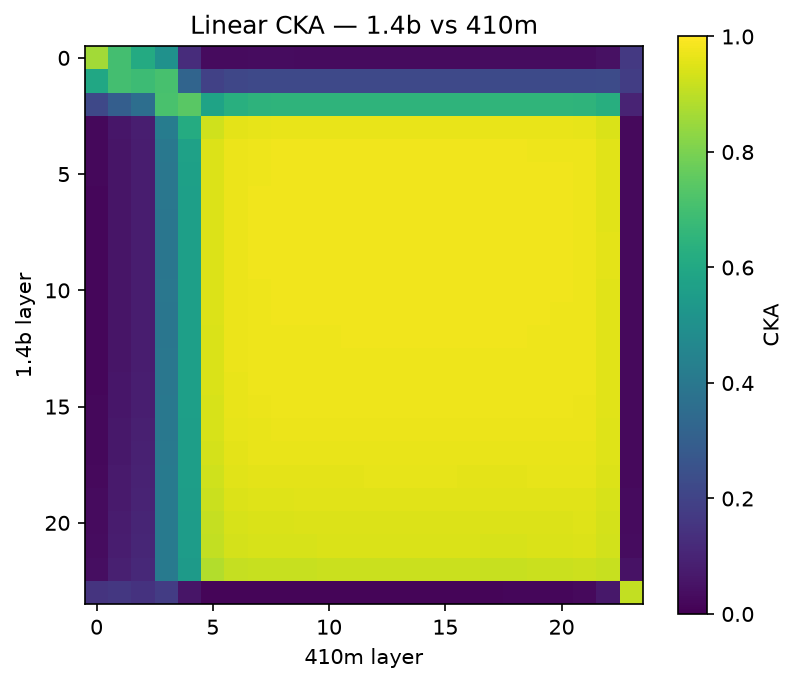
\includegraphics[width=0.46\linewidth]{figures/cka_heatmap.png}
\hfill
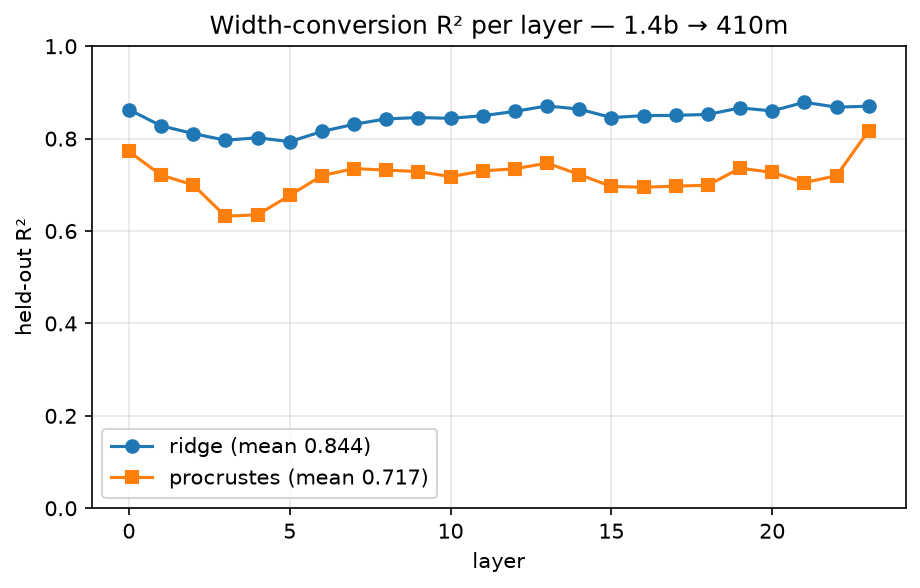
\includegraphics[width=0.46\linewidth]{figures/maps_r2.png}
\caption{Alignment across sizes for the primary pair (1.4B$\,\to\,$410M).
\textbf{(left)} Linear CKA between all $24\times24$ layer pairs: a saturated
middle band (layers $\sim$4--22 mutually $\approx1.0$) confirms coarse
correspondence but resolves no sharp per-layer match. \textbf{(right)} Held-out
$R^2$ of the per-layer activation maps: ridge (full linear) and Procrustes
(rotation$+$scale) track each other and dip together at layers 3--5, the layers
CKA also flags as distinct.}
\label{fig:align}
\end{figure}

\begin{table}[h]
\centering
\caption{Alignment across sizes, held-out. Activations align strongly under a
linear map; raw parameters, even in the cleanest (embedding) case, do not.
Best (highest) map per row in \textbf{bold}.}
\label{tab:align}
\begin{tabular}{lccc}
\toprule
Target & CKA & Ridge $R^2$ & Procrustes $R^2$ \\
\midrule
Pooled activations (per-layer mean) & $0.883^{\dagger}$ & \textbf{0.844} & 0.717 \\
\midrule
Input embedding & 0.512 & \textbf{0.248} & 0.167 \\
Output embedding (unembedding) & 0.678 & \textbf{0.386} & 0.242 \\
\bottomrule
\end{tabular}
\\[3pt]
{\footnotesize $^{\dagger}$ For activations, the diagonal mean of the
$24\times24$ linear-CKA matrix, which saturates in the middle band
(Figure~\ref{fig:align}, left); for embeddings, linear CKA before mapping.}
\end{table}

\subsection{Projection diagnostics (\S\ref{sec:projection})}
\label{app:projection}

\begin{table}[h]
\small
\begin{minipage}[t]{0.55\linewidth}
\centering
\caption{Relative Frobenius error of projected weights vs.\ the actual 410M
weights (mean over 24 layers). Every target-free error exceeds $1$ (worse than
zero); lower per row in \textbf{bold}.}
\label{tab:proj}
\setlength{\tabcolsep}{4pt}
\begin{tabular}{lcc}
\toprule
Weight & Projection & Operator$^{\dagger}$ \\
       & (target-free) & (fitted) \\
\midrule
$Q$            & 1.471 & \textbf{0.658} \\
$K$            & 1.591 & \textbf{0.758} \\
$V$            & 1.390 & \textbf{0.804} \\
$O$            & 1.724 & \textbf{0.795} \\
\texttt{MLP\_UP}   & 1.668 & \textbf{0.683} \\
\texttt{MLP\_DOWN} & 1.723 & \textbf{0.686} \\
\bottomrule
\end{tabular}
\\[3pt]
{\footnotesize $^{\dagger}$ A single $(A,B)$ shared across layers per type; it
peeks at the target and so upper-bounds the linearly explainable fraction. A
\emph{per-layer} fit is degenerate (error $\to 0$ around any full-rank $W$) and
is not reported.}
\end{minipage}\hfill
\begin{minipage}[t]{0.43\linewidth}
\centering
\caption{Zero-shot dense-projected quality (strided WikiText-103 perplexity);
the projected model does not beat random init. Best (lowest) in \textbf{bold}.}
\label{tab:anchor}
\begin{tabular}{lc}
\toprule
Model & Perplexity \\
\midrule
real 1.4B (reference)        & \textbf{11.5} \\
real 410M (upper anchor)     & 15.6 \\
random-init 410M (lower)     & 65{,}962 \\
\midrule
proj., LN from 410M   & 181{,}242 \\
proj., LN from 1.4B & $10^{13}$ \\
\bottomrule
\end{tabular}
\\[3pt]
{\footnotesize With fresh \emph{neutral} LayerNorms (gain 1, bias 0) the same
projected matrices score $\sim$12.3k quick-perplexity --- $\sim$15$\times$ better
than the 181{,}242 row and $\sim$5$\times$ better than random init --- so much of
the collapse is LayerNorm mismatch, not weight destruction alone
(\S\ref{sec:race}); the structure-mixing diagnosis still holds directionally.}
\end{minipage}
\end{table}

\subsection{Spectral residual test (\S\ref{sec:residuals})}
\label{app:spectral}

\begin{table}[h]
\centering
\caption{Test 1 (spectral). Effective rank of the residual $\Delta$ vs.\ a
per-type shuffled control and a shape/scale-matched Gaussian control. $\Delta$
sits $2.8$--$6.4\%$ below both in every type --- a faint, non-isotropic
concentration, not a learnable direction.}
\label{tab:erank}
\begin{tabular}{lccc}
\toprule
Weight & $\Delta$ erank & Shuffled & Gaussian \\
\midrule
$Q$            & 771.3 & 824.1 & 824.1 \\
$K$            & 784.0 & 824.0 & 824.1 \\
$V$            & 801.2 & 824.2 & 824.1 \\
$O$            & 792.2 & 824.1 & 824.1 \\
\texttt{MLP\_UP}   & 947.2 & 989.4 & 989.4 \\
\texttt{MLP\_DOWN} & 934.8 & 989.4 & 989.4 \\
\bottomrule
\end{tabular}
\end{table}

\begin{figure}[h]
\centering
% source: results/m4_residuals/*/delta_spectra.png (gitignored, regenerable)
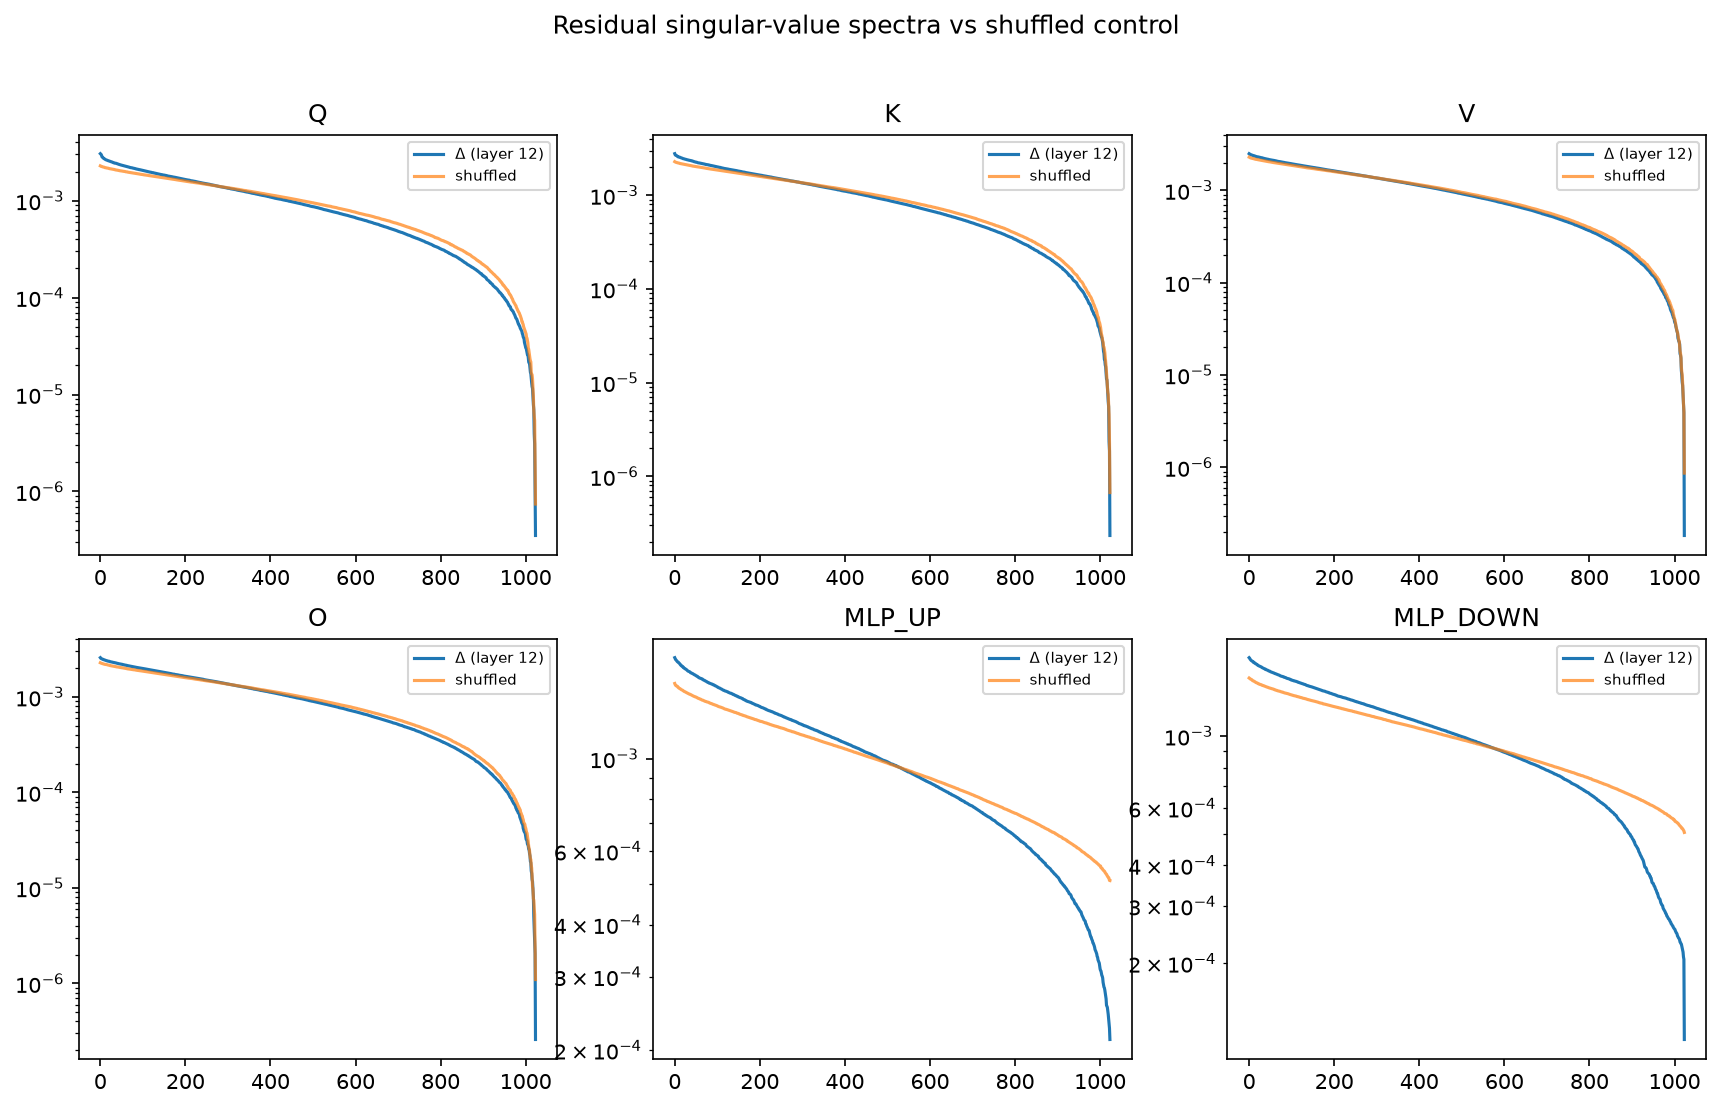
\includegraphics[width=0.6\linewidth]{figures/delta_spectra.png}
\caption{Test 1 (spectral). Singular-value spectrum of the residual $\Delta$
against shuffled and Gaussian controls. $\Delta$ concentrates $2.8$--$6.4\%$ more
than either control in every weight type --- a faint, generic non-isotropy that
carries no layer-specific, predictable signal (Table~\ref{tab:predictor}).}
\label{fig:spectra}
\end{figure}

\subsection{Extended evaluation, primary pair (\S\ref{sec:race:hardening})}
\label{app:extended}

\begin{table}[h]
\centering
\caption{Extended evaluation of the 30M primary-pair checkpoints and the
real-410M reference. Guess floors: arc\_easy $0.25$, hellaswag $0.25$, piqa
$0.50$, lambada $\approx0$ (open-vocabulary). Best converted arm in
\textbf{bold}; the ordering holds on all six metrics. Single-seed checkpoints.
This table predates the rescale-lever ablation and reports the compensation
contrast (\textsc{hybrid} vs.\ \textsc{subclone}); the rescale gains of
Tables~\ref{tab:ladder}--\ref{tab:seeded} stack on top of it.}
\label{tab:extended}
\begin{tabular}{lrrrrrr}
\toprule
Model & C4 ppl & wk@2048 & lambada & arc\_easy & hellaswag & piqa \\
\midrule
\textbf{hybrid} & \textbf{90.7} & \textbf{109.8} & \textbf{0.076} & \textbf{0.313} & \textbf{0.266} & \textbf{0.555} \\
subclone        & 162.7 & 346.3 & 0.005 & 0.308 & 0.263 & 0.548 \\
projection      & 380.5 & 1{,}210 & 0.000 & 0.272 & 0.258 & 0.539 \\
random          & 518.8 & 1{,}788 & 0.000 & 0.264 & 0.256 & 0.532 \\
\midrule
real 410M       & 21.0 & 14.5 & 0.516 & 0.519 & 0.337 & 0.667 \\
\bottomrule
\end{tabular}
\end{table}

\subsection{Primary-pair seeded verdict (\S\ref{sec:race:seeded})}
\label{app:seeded}

\begin{table}[h]
\centering
\footnotesize
\caption{Primary-pair final WikiText-103 perplexity across three data-draw seeds
(30M tokens; identical budget/schedule per seed). \textsc{hybrid\_rs} wins every
paired comparison; its worst seed beats \textsc{subclone\_rs}'s best.}
\label{tab:seeded}
\begin{tabular}{lrrrr}
\toprule
Init & seed 0 & seed 1 & seed 2 & mean $\pm$ std \\
\midrule
subclone\_rs        & 86.4 & 93.7 & 88.9 & $89.7 \pm 3.7$ \\
\textbf{hybrid\_rs} & \textbf{83.0} & \textbf{86.0} & \textbf{82.8} & $\mathbf{84.0 \pm 1.8}$ \\
\bottomrule
\end{tabular}
\end{table}

\subsection{Held-out pair per-seed detail (\S\ref{sec:race:hardening})}
\label{app:unseen}

\begin{table}[h]
\centering
\caption{Held-out pair (410M$\to$160M), final WikiText-103 perplexity across
three data-draw seeds (30M tokens). Transfer beats from scratch $\sim$$13\times$
on every seed; hybrid and subclone are a statistical tie on this
depth-dominated pair (overlapping $\pm1\sigma$).}
\label{tab:unseen}
\begin{tabular}{lrrrr}
\toprule
Init & seed 0 & seed 1 & seed 2 & mean $\pm$ std \\
\midrule
\textbf{hybrid} & 117.5 & 113.6 & 108.5 & $\mathbf{113.2 \pm 4.5}$ \\
subclone        & 115.0 & 121.6 & 118.9 & $118.5 \pm 3.3$ \\
random          & 1{,}464.4 & 1{,}571.5 & 1{,}479.6 & $1{,}505.2 \pm 57.9$ \\
\bottomrule
\end{tabular}
\end{table}

\paragraph{Metric robustness (held-out pair).}
\label{app:unseen-metrics}
On the held-out 410M$\to$160M pair the hybrid-vs-subclone tie holds on every
metric beyond WikiText-103: C4 perplexity $91.1$ vs.\ $94.2$, perplexity at
$2\times$ context $111.8$ vs.\ $110.2$, LAMBADA $11.0\%$ vs.\ $10.7\%$ (others
within noise), while random sits at C4 $514$ and LAMBADA $0$; the real-160M
anchor (LAMBADA $35.4\%$) matches published Pythia numbers. These cells are
single-seed.

\begin{figure}[h]
\centering
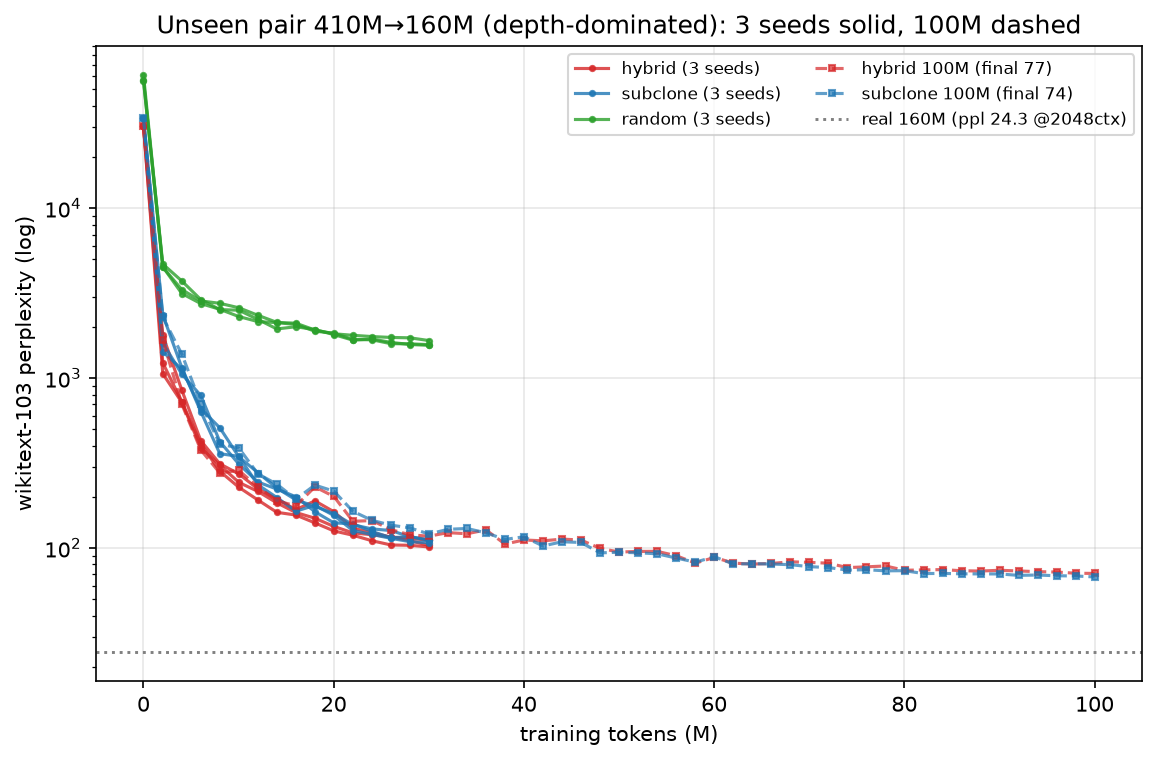
\includegraphics[width=0.92\linewidth]{figures/m5b_curves.png}
\caption{\textbf{Held-out pair (410M$\to$160M), three seeds.} Full WikiText-103
perplexity (log scale) versus tokens; bands span the three data-draw seeds and
the dashed line marks the real Pythia-160M reference. Transfer inits (hybrid,
subclone) sit an order of magnitude below random throughout and overlap each
other --- the depth-dominated regime where compensation's width-repair edge is
neutral (Table~\ref{tab:unseen}), yet the $\sim$$13\times$ margin over from
scratch is preserved on every seed.}
\label{fig:m5bcurves}
\end{figure}

\subsection{Scale pair (\S\ref{sec:race:scale})}
\label{app:scale}

\begin{table}[h]
\centering
\caption{Scale pair (6.9B$\to$1.4B), 30M tokens, single seed. The two levers that
stack at smaller scale here \emph{anti}-synergize --- each alone beats the
combination --- though every transfer arm still beats from scratch
(\S\ref{sec:race:scale}).}
\label{tab:scale}
\begin{tabular}{llr}
\toprule
Init & Construction & Final ppl (30M) \\
\midrule
random       & from scratch             & 1{,}413 \\
hybrid\_rs   & compensation $+$ rescale & 1{,}213 \\
hybrid       & compensation only        & 776 \\
subclone\_rs & rescale only             & \textbf{572} \\
\bottomrule
\end{tabular}
\end{table}

\section{Deferred discussion}
\label{app:discussion}

\subsection{An honest correction (\S\ref{sec:race:seeded})}
\label{app:correction}

The rescale lever corrects our own earlier reading. When the hybrid first won at
$114.1$ we argued that least-squares compensation \emph{subsumed} the reference
recipe's scalar rescale, since a ridge-optimal map beats a scalar on the paths it
re-fits. The upset --- \textsc{subclone\_rs} at $86.4$, beating the hybrid with no
compensation --- showed that is only half right: compensation dominates rescale
\emph{on the two read-out paths it touches}, but the LN-fronted read-in paths it
leaves alone still benefit from the reference recipe's variance correction as a
training-dynamics prior. Blanket rescale collapses zero-shot yet wins on
dynamics, so the reference recipe is vindicated exactly where our first account
wrote it off, and the principled method is the stack, not either lever alone.

\subsection{Reconciling the faint spectral signal (\S\ref{sec:residuals})}
\label{app:reconcile}

Tests 1 and 3 are not in tension: the $2.8$--$6.4\%$ spectral deficit is a
\emph{generic} statistical trace (mild row/column-norm heterogeneity), not a
correspondence between $\hat{W}$ and $\Delta$ any predictor can exploit. A
behavioral cross-check agrees: an assembled 410M whose six matrix types are
operator-projected (with real biases, LayerNorms, and embeddings) scores
$35{,}212$ perplexity, and the learned correction moves it only $\sim$2\% (to
$34{,}373$); both remain non-functional. Notably the operator matrices alone beat
random init ($35$k vs.\ $66$k) once the surrounding tensors are real --- unlike
\S\ref{sec:projection}'s fully projected model --- again locating the destruction
in the dense projection, not the residual. (The correction's gains on the 18
training layers are partly memorized; only the held-out layers carry genuine
predictions, and there the reduction is zero.)

\section{Training protocol details}
\label{app:protocol}

Every conversion arm within an experiment shares \emph{identical} data order,
optimizer (AdamW, $\beta=(0.9,0.95)$, weight decay $0.1$), cosine schedule
with 100-step warmup, gradient clipping at $1.0$, bf16 autocast, and token
budget (30M primary; 100M persistence checks); the learning rate equals the
target size's original pretraining rate. Initialization construction costs
are negligible against any training budget (selection: seconds; moments pass
for compensation: $\sim$75\,s; closed-form solves: seconds) and are included
in the compute accounting. All experiments ran on a single NVIDIA GB10
(128\,GB unified memory); any 24\,GB+ CUDA GPU reproduces them.


\end{document}
